\documentclass[international_finance_p1.tex]{subfiles}

\begin{document}
\setbeamercovered{transparent}
\section{The Foreign Exchange Market}
\subsection{Forex definition}
\begin{frame}{Foreign Exchange Market definition}
\begin{block}{The foreign exchange market }
is a place where large commercial banks trade foreign-currency-denominated deposits with each other.
The foreign exchange market (forex, FX, or currency market) is a global decentralized market for the trading of currencies. This includes all aspects of buying, selling and exchanging currencies at current or determined prices.
\end{block}
The modern foreign exchange market began forming during the 1970s after three decades of government restrictions on foreign exchange transactions.
\end{frame}
\begin{frame}{The foreign exchange market characteristics}
\begin{itemize}[<+->]
\item
huge trading volume representing the largest asset class in the world leading to high liquidity;
\item
geographical dispersion;
\item
continuous operation: 24 hours a day except weekends, i.e., trading from 22:00 GMT on Sunday (Sydney) until 22:00 GMT Friday (New York);
\item
the variety of factors that affect exchange rates;
\item
the low margins of relative profit compared with other markets of fixed income; 
\item
the use of leverage to enhance profit and loss margins with respect to account size.
\end{itemize}
\end{frame}

\begin{frame}[shrink=15]{The size of the Forex market}
% Table generated by Excel2LaTeX from sheet 'Лист1'
\begin{table}[htbp]
  \centering
  \fontsize{10pt}{10pt}\selectfont
  \caption{Global foreign exchange market turnover,\\
daily averages in billions of US dollars and percentages}
\begin{tabularx}{\linewidth}[b]{@{}>{\raggedright\arraybackslash}Xrrrrrr@{}}
	\toprule
	Instrument                            & 1998 & 2001 & 2004 & 2007 & 2010 & 2013 \\ \midrule
	\textbf{Foreign exchange instruments} & 1527 & 1239 & 1934 & 3324 & 3971 & 5345 \\
	Spot transactions                     & 37\% & 31\% & 33\% & 30\% & 37\% & 38\% \\
	Outright forwards                     & 8\%  & 10\% & 11\% & 11\% & 12\% & 13\% \\
	Foreign exchange swaps                & 48\% & 53\% & 49\% & 52\% & 44\% & 42\% \\
	Currency swaps                        & 1\%  & 1\%  & 1\%  & 1\%  & 1\%  & 1\%  \\
	Options and other products            & 6\%  & 5\%  & 6\%  & 6\%  & 5\%  & 6\%  \\ \bottomrule
\end{tabularx}%
  \label{tab:addlabel}%
\end{table}%

Source: Bank for International Settlements. Triennial Central Bank Survey. Report on Global Foreign Exchange Market Activity in 2013. Basel, December, 2013.

\end{frame}
\begin{frame}[shrink=15]
% Table generated by Excel2LaTeX from sheet 'Лист2'
\begin{table}[htbp]
  \centering
  \fontsize{10pt}{10pt}\selectfont  
  \caption{Global foreign exchange market turnover by currency pair,\\daily averages in billions of US dollars and percentages}
\begin{tabularx}{\linewidth}[b]{@{}>{\raggedright\arraybackslash}Xrrr@{}}
	\toprule
	          & 2001         & 2007         & 2013          \\ \midrule
	USD / EUR & 372 (30\%)   & 892 (26,8\%) & 1289 (24,1\%) \\
	USD / JPY & 250 (20,2\%) & 438 (13,2\%) & 978 (18,3\%)  \\
	USD / GBP & 129 (10,4\%) & 384 (11,6\%) & 472 (8,8\%)   \\
	USD / AUD & 51 (4,1\%)   & 185 (5,6\%)  & 364 (6,8\%)   \\
	USD / CAD & 54 (4,3\%)   & 126 (3,8\%)  & 200 (3,7\%)   \\
	USD / CHF & 59 (4,8\%)   & 151 (4,5\%)  & 184 (3,4\%)   \\
	USD / OTH & 199 (16\%)   & 612 (18,4\%) & 213 (4\%)     \\
	EUR / JPY & 36 (2,9\%)   & 86 (2,6\%)   & 147 (2,8\%)   \\
	EUR / GBP & 27 (2,1\%)   & 69 (2,1\%)   & 102 (1,9\%)   \\
	EUR / CHF & 13 (1,1\%)   & 62 (1,9\%)   & 71 (1,3\%)    \\
	EUR / OTH & 20 (1,6\%)   & 83 (2,5\%)   & 52 (1\%)      \\ \midrule
	All pairs & 1239 (100\%) & 3324 (100\%) & 5345 (100\%)  \\ \bottomrule
\end{tabularx}%
  \label{tab:addlabel}%
  
\raggedright
  \small{Source: Bank for International Settlements. Triennial Central Bank Survey. Report on Global Foreign Exchange Market Activity in 2013. Basel, December, 2013.}
\end{table}%


\end{frame}
\begin{frame}[shrink=15]
% Table generated by Excel2LaTeX from sheet 'Лист3'
\begin{table}[htbp]
  \centering
  \fontsize{10pt}{10pt}\selectfont  
  \caption{Geographical distribution\\of global foreign exchange market turnover,\\2 daily averages in billions of US dollars and percentages}
\begin{tabularx}{\linewidth}[b]{@{}>{\raggedright\arraybackslash}Xrrr@{}}
	\toprule
	               & 2004         & 2010          & 2013          \\ \midrule
	United Kingdom & 835 (32\%)   & 1854 (36,8\%) & 2726 (40,9\%) \\
	United States  & 499 (19,1\%) & 904 (17,9\%)  & 1263 (18,9\%) \\
	Singapore      & 134 (5,1\%)  & 266 (5,3\%)   & 383 (5,7\%)   \\
	Japan          & 207 (8\%)    & 312 (6,2\%)   & 374 (5,6\%)   \\
	Hong Kong SAR  & 106 (4,1\%)  & 238 (4,7\%)   & 275 (4,1\%)   \\
	Switzerland    & 85 (3,3\%)   & 249 (4,9\%)   & 216 (3,2\%)   \\ \midrule
	Total          & 2608 (100\%) & 5043 (100\%)  & 6671 (100\%)  \\ \bottomrule
\end{tabularx}%
  \label{tab:addlabel}%

\raggedright
\small{Source: Bank for International Settlements. Triennial Central Bank Survey. Report on Global Foreign Exchange Market Activity in 2013. Basel, December, 2013.}
\end{table}%
\end{frame}

\subsection{International Market participants}
\begin{frame}{}
\begin{itemize}[<+->]
\item
The interbank market: the largest commercial banks and securities dealers.
\item
Commercial companies.
\item
Central banks.
\item
Hedge funds.
\item
Investment management firms.
\item
Retail foreign exchange traders.
\item
Non-bank foreign exchange companies.
\item
Money transfer/remittance companies and bureaux de change.
\end{itemize}
\end{frame}
\begin{frame}[shrink=10]{Market maker}
\begin{block}{\textbf{A market maker}}
or liquidity provider is a company, or an individual, that quotes both a buy and a sell price in a financial instrument or commodity held in inventory, hoping to make a profit on the bid-offer spread, or turn.
\end{block}
\begin{itemize}[<+->]
\item
The U.S. Securities and Exchange Commission defines a "market maker" as a firm that stands ready to buy and sell stock on a regular and continuous basis at a publicly quoted price.
\item
A Designated Primary Market Maker (DPM) is a specialized market maker approved by an exchange to guarantee that he or she will take the position in a particular assigned security, option or option index
\end{itemize}
\end{frame}
\begin{frame}{Large market makers}
\textbf{General forex}: Barclays Bank Plc (LSE: BARC.L), JPMorgan Chase \& Co (JPM), Union Bank of Switzerland (UBS), Mizuho Financial Group, Inc. (MHFG), Deutsche Bank AG (DBK)

\textbf{USD/CHF}: Union Bank of Switzerland (UBS), Credit Suisse Group (CS.N).

\textbf{Exotic currencies}: Standard Chartered Bank (STAN.L).
Russian ruble: Alfabank, Sberbank ect.

\end{frame}
\begin{frame}{Financial markets information}
\begin{itemize}[<+->]
\item
Reuters
\item
Dow Jones 
\item
Bloomberg
\end{itemize}
\end{frame}

\subsection{Financial centres}
\begin{frame}[shrink=10]{Financial centres}
\begin{block}{A financial centre}
 is a location that is home to a cluster of nationally or internationally significant financial services providers such as banks, investment managers or stock exchanges. 
\end{block}
\begin{block}{The International Monetary Fund definition}
    International Financial Centers (IFCs)—such as London, New York, and Tokyo—are large international full-service centers with advanced settlement and payments systems, supporting large domestic economies, with deep and liquid markets where both the sources and uses of funds are diverse, and where legal and regulatory frameworks are adequate to safeguard the integrity of principal-agent relationships and supervisory functions.
\end{block}
\end{frame}
\begin{frame}[shrink=20]
\begin{figure}	
	\centering
	\begin{subfigure}[t]{5.1cm}
		\centering
		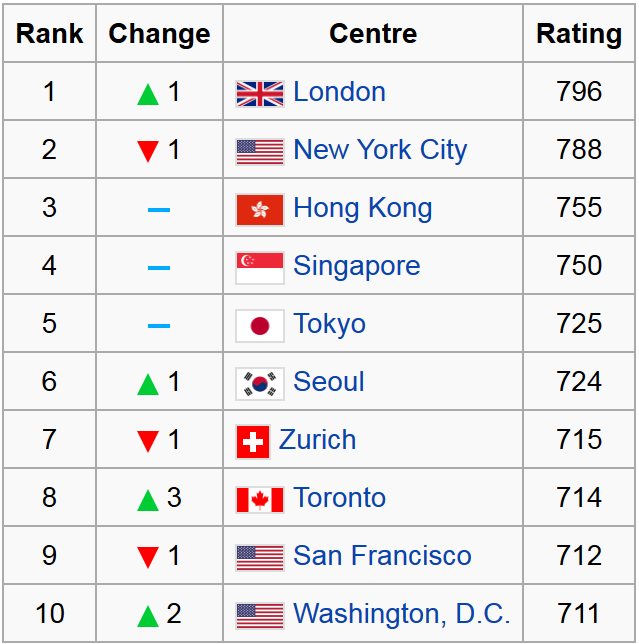
\includegraphics[scale=0.4]{img/financial_centers_ranking1.png}
	\caption{Global Financial Centres Index (GFCI)}\label{fig:a_fin_centers_index}	
	\end{subfigure}
	\quad
	\begin{subfigure}[t]{5.1cm}
		\centering
		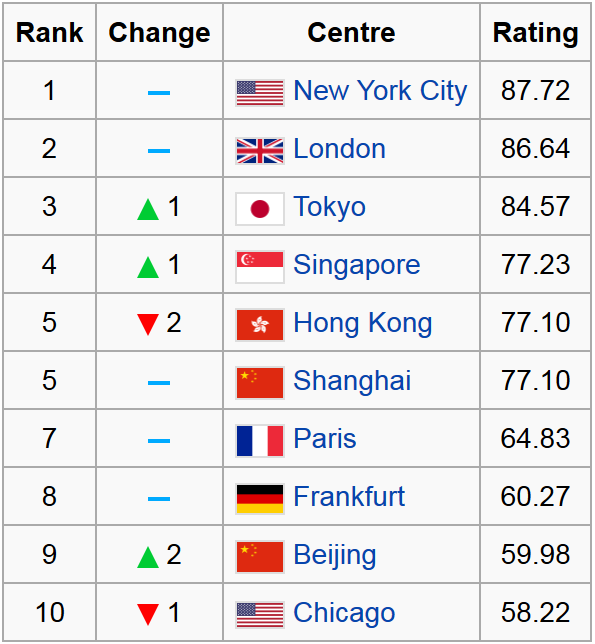
\includegraphics[scale=0.4]{img/financial_centers_ranking2.png}
		\caption{International Financial Centres Development Index (IFCDI)}\label{fig:b_fin_centers_index}
	\end{subfigure}
	\caption{Financial Centres ranking}\label{fig:df_and_cdf}
\end{figure}
\footnotesize{GFCI - London-based British think-tank Z/Yen, Qatar Financial Centre Authority;

IFCDI - The Xinhua News Agency of China, The Chicago Mercantile Exchange and Dow Jones Company of the United States.}
\end{frame}

\begin{frame}
\begin{figure}
\centering
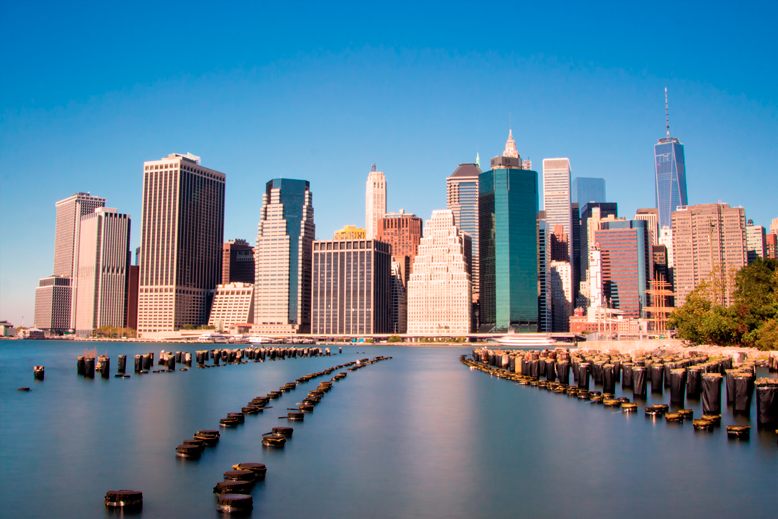
\includegraphics[scale=0.25]{img/new_york}
\caption{New York City's Financial District in Lower Manhattan, which includes Wall Street. Many financial firms have expanded northward to Midtown Manhattan.}
\end{figure}
\end{frame}

\begin{frame}
\begin{figure}
\centering
\fontsize{8pt}{8pt}\selectfont
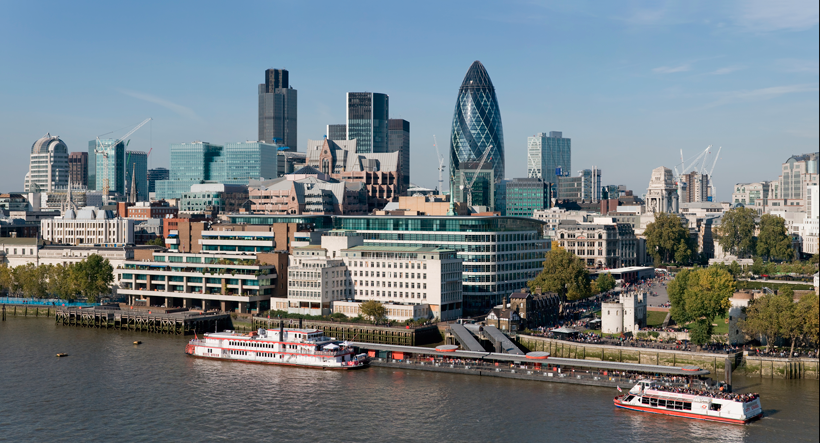
\includegraphics[scale=0.5]{img/london}
\caption{The City of London is one of the oldest financial centres and today remains at the heart of London's financial services industry}
\end{figure}
\end{frame}
\begin{frame}
\begin{figure}
\centering
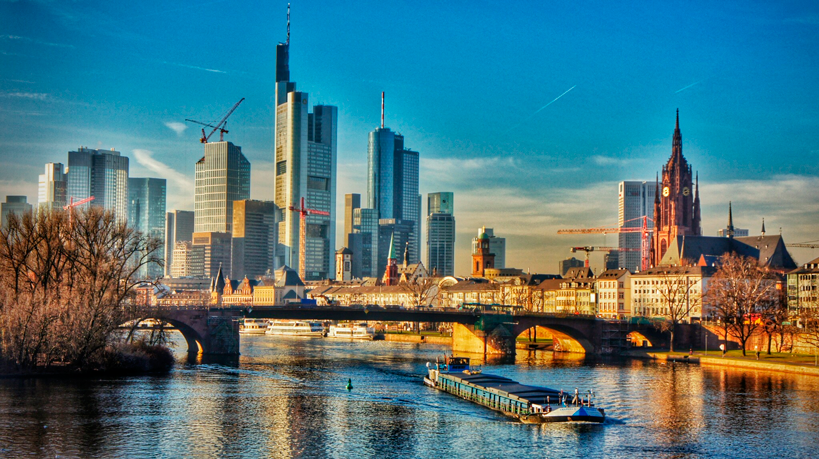
\includegraphics[scale=0.3]{img/frankfurt}
\caption{Frankfurt's banking district, home of the European Central Bank.}
\end{figure}
\end{frame}
\begin{frame}
\begin{figure}
\centering
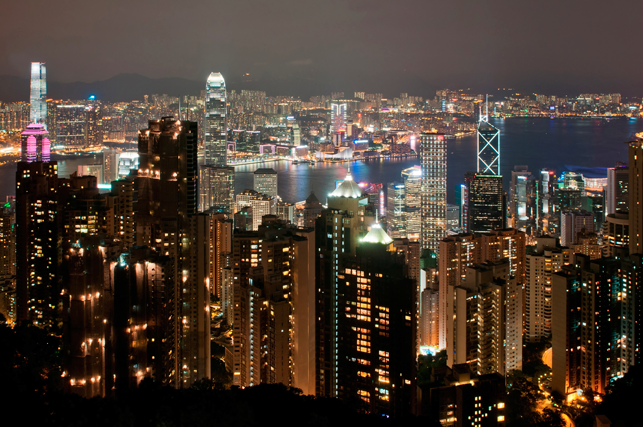
\includegraphics[scale=0.35]{img/Hong_Kong}
\caption{The Central District of Hong Kong, one of the main financial centres in Asia}
\end{figure}
\end{frame}


\subsection{Currency quote}
\begin{frame}{Understanding currency quote}
\begin{itemize}[<+->]
\item
When a currency is quoted, it is done in relation to another currency, so that the value of one is reflected through the value of another. 
\item
 USD/JPY = 102.50.
\item
The base currency is set to the left of the slash, while the currency on the right is referred to as the quote or counter currency
\end{itemize}
\end{frame}
\begin{frame}{Direct and indirect quote}
\begin{itemize}[<+->]
\item
In a direct currency quote the domestic currency is the base currency. The direct quote varies the foreign currency, and the quoted, or domestic currency, remains fixed at one unit.
\item
In an indirect quote the domestic currency is the quoted currency. The domestic currency is variable and the foreign currency is fixed at one unit.
\end{itemize}
\end{frame}
\begin{frame}{}
\begin{itemize}[<+->]
\item
U.S. dollar as a base currency in the currency pair.
\item
The Queen's currencies: the British pound, Australian Dollar and New Zealand dollar - are all quoted as the base currency against the U.S. dollar. The euro is quoted the same way as well.
\end{itemize}
\end{frame}
\begin{frame}{Example of the currency quotes}
\begin{figure}
\centering
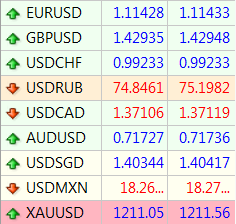
\includegraphics[scale=0.7]{img/currency_quotes}
\caption{Currency quotes example}
\end{figure}
Most currency exchange rates are quoted out to five digits after the decimal place, with the exception of the Japanese yen (JPY), which is quoted out to three decimal places.
\end{frame}

\begin{frame}{Cross currency pairs}
\begin{itemize}[<+->]
\item
When a currency quote is given without the U.S. dollar as one of its components, this is called a cross currency. The most common cross currency pairs are the EUR/GBP, EUR/CHF and EUR/JPY.
\end{itemize}
\end{frame}
\begin{frame}{Bid and Ask price}
\begin{itemize}[<+->]
\item
When buying a currency pair (going long), the ask price refers to the amount of quoted currency that has to be paid in order to buy one unit of the base currency, or how much the market will sell one unit of the base currency for in relation to the quoted currency.
\item
When selling a currency pair (going short) the bid price reflects how much of the quoted currency will be obtained when selling one unit of the base currency, or how much the market will pay for the quoted currency in relation to the base currency.
\end{itemize}
\end{frame}
\begin{frame}{}
Whichever currency is quoted first (the base currency) is always the one in which the transaction is being conducted. Operator either buys or sells the base currency.
\end{frame}
\begin{frame}{Spread, pips and points}
\begin{itemize}[<+->]
\item
The difference between the bid price and the ask price.
\item
EUR/USD = 1.25155/035, the spread would be 0.00035 or 35 pips, also known as points.
\item
The pip is the smallest amount a price can move in any currency quote. In the case of the U.S. dollar, euro, British pound or Swiss franc, one pip would be 0.00001. With the Japanese yen, one pip would be 0.001, because this currency is quoted to two decimal places.
\end{itemize}
\end{frame}
\subsection{Long and short positions}
\begin{frame}[shrink=15]{Long and short positions}
\begin{itemize}[<+->]
\item
\textbf{A long position }in a security, such as a stock or a bond, or equivalently to be long in a security, means the holder of the position owns the security and will profit if the price of the security goes up. 
\item
\textbf{Short selling }(also known as shorting or going short) is the practice of selling securities or other financial instruments that are not currently owned, and subsequently repurchasing them ("covering").
\item
\textbf{Net position} is the difference between total open long (receivable) and open short (payable) positions in a given asset (security, foreign exchange currency, commodity, etc.) held by an individual. This also refers to the amount of assets held by a person, firm, or financial institution, as well as the ownership status of a person's or institution's investments.
\end{itemize}
\end{frame}
\begin{frame}{Short positions on the stock exchange}
\begin{figure}
	\centering
	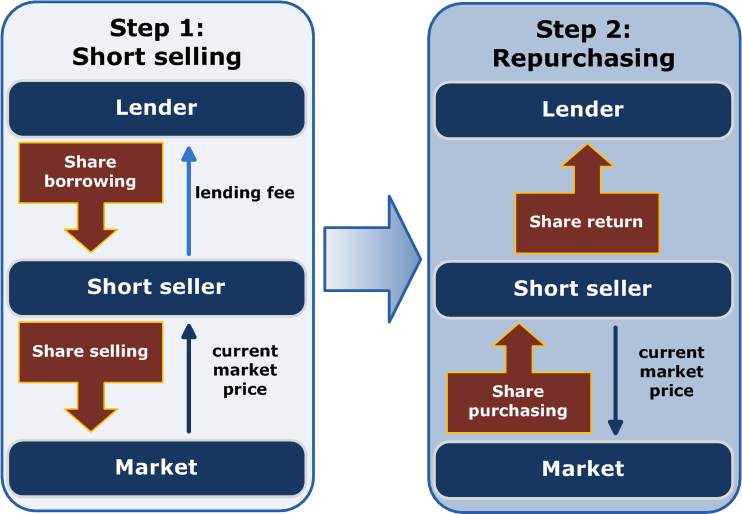
\includegraphics[scale=0.3]{img/shortselling.png}
	\caption{Short trade scheme}
\end{figure}

\end{frame}
\begin{frame}[shrink=15]{Sources of short interest data}
\begin{itemize}[<+->]
\item
Time delayed short interest data (for legally shorted shares) is available in a number of countries, including the US, the UK, Hong Kong, and Spain. 
\item
The number of stocks being shorted on a global basis has increased in recent years for various structural reasons
\item
Market data providers (Data Explorers, SunGard Financial Systems) believe that stock lending data provides a good proxy for short interest levels (excluding any naked short interest). 
\item
SunGard provides daily data on short interest by tracking the proxy variables based on borrowing and lending data which it collects.
\end{itemize}
\end{frame}
\begin{frame}{Selling short on the currency markets }
\begin{itemize}[<+->]
\item
Currencies are traded in pairs, each currency being priced in terms of another. In this way, selling short on the currency markets is identical to going long on stocks.
\item
A contract is always long in terms of one medium and short another.
\item
When the exchange rate has changed, the trader buys the first currency again; this time he gets more of it, and pays back the loan. Since he got more money than he had borrowed initially, he makes money.
\end{itemize}
\end{frame}
\begin{frame}
% Table generated by Excel2LaTeX from sheet 'Лист3'
\begin{table}[htbp]
  \centering
  \tiny
  \caption{Bank trades during the day}
\begin{tabularx}{\linewidth}[b]{@{}>{\raggedright\arraybackslash}XXcXX@{}}
	\toprule
	              \multicolumn{2}{c}{Currency trade}               & $R_E$  & \multicolumn{2}{c}{Currency position} \\
	\cmidrule{1-2} \cmidrule{4-5}
    Bought      & Sold           &        & Long        & Short                   \\
	\cmidrule{1-2} \cmidrule{4-5}
    100 000 EUR & 119 040 USD    & 1.1904 & 100 000 EUR & 119 040 USD             \\
	100 000 USD                                   & 11 785 000 JPY & 117.85 & 100 000 USD & 11 785 000 JPY          \\
	122 087 USD                                   & 70 000 GBP     & 1.7441 & 122 087 USD & 70 000 GBP              \\ \midrule
	\multicolumn{3}{l}{\multirow{2}[0]{*}{Net position}}                    & 103 047 USD & 11 785 000 JPY          \\
	\multicolumn{3}{l}{}                                                    & 100 000 EUR & 70 000 GBP              \\ \bottomrule
\end{tabularx}%
  \label{tab:addlabel}%
\end{table}%
% Table generated by Excel2LaTeX from sheet 'Лист3'
\begin{table}[htbp]
  \centering
  \tiny
  	\caption{Next day currency quotes}
    \begin{tabular}{rrl}
    \toprule
    EURUSD & 1,2023 & Bank closes down long EUR \\
    USDJPY & 119.1464 & Bank closes down short JPY \\
    GBPUSD & 1,7371 & Bank closes down short GPB \\
    \bottomrule
    \end{tabular}%
  \label{tab:addlabel}%
\end{table}%
\end{frame}
\setbeamercovered{invisible}
\begin{frame}{Solution}
\begin{align*}
\onslide<2->{100000EUR\cdot(1.2023-1.1904)&=}\onslide<3->{1190USD\\}
\onslide<4->{-11785000JPY\cdot(\frac{1}{119.1464}-\frac{1}{117.85})&=}\onslide<5->{1087.74USD\\}
\onslide<6->{-70000GBP\cdot(1.7371-1.7441)&=}\onslide<7->{490USD}
\end{align*}
\end{frame}
\setbeamercovered{transparent}
\subsection{Currency Arbitrage}
\setbeamercovered{invisible}
\begin{frame}{Currency Arbitrage}
\begin{block}{Currency arbitrage}
 is the practice of taking advantage of exchange rates difference between two or more markets
\end{block}
Arbitrage opportunity for USD/CHF:
Citibank is quoting 0.8745-55.
Deutsche Bank is quoting 0.8725-35.
\begin{itemize}[<+->]
\item
Trader could buy USD10 mln at Deutsche Bank’s offer price of 0.8735 and simultaneously sell USD10 mln to Citibank at their bid price of 0.8745 francs. 
\item
This would earn a profit of SF0.0010 per dollar traded, or SF10,000 would be the total arbitrage profit.
\end{itemize}
\end{frame}
\begin{frame}{Triangular arbitrage}
% Table generated by Excel2LaTeX from sheet 'Triangular currency arbitrage'
\begin{table}[htbp]
  \centering
\begin{tabularx}{\linewidth}[b]{@{}>{\raggedright\arraybackslash}Xrrr@{}}    \toprule
          & USDCHF & GBPUSD & GBPCHF \\
    \midrule
    New York & 0,9987 & 1,3947 & \onslide<2-> {1,3929} \\
    London & \multicolumn{1}{c}{--} & 1,3947 & 1,3920 \\
    Geneva & 0,9987 & \multicolumn{1}{c}{--} & 1,3920 \\
    \bottomrule
    \end{tabularx}%
  \label{tab:addlabel}%
  \caption*{Table appears to have no possible arbitrage opportunity.}
\end{table}%
\onslide<2-> Computing the implicit cross rate for New York, the arbitrageur finds the implicit cross rate to be $GBPCHF = 0,9987 \cdot 1,3947 = 1,3929.$

Thus the cost of GBP is high in New York, and the cost of CHF is low.
\end{frame}
\setbeamercovered{transparent}
\subsection{Short-term  and Long-term Forex Movements}
\begin{frame}{Short-term  and Long-term Foreign Exchange Movements}
\begin{itemize}
\item
Causes of short-term (throughout the day) FX movements:
	\setbeamertemplate{items}[circle]
	\begin{itemize}
		\item
		inventory control;
		\item
		asymmetric information effects.
	\end{itemize}
\setbeamertemplate{items}[square]
\item
In the long run, economic factors affect the exchange rate movements:
	\setbeamertemplate{items}[circle]
	\begin{itemize}
	\item
	demand/ supply of foreign and domestic goods);
	\item
	Government policy change;
	\item
	Economic growth and inflation.
	\end{itemize}
\end{itemize}

\end{frame}
\subsection{Russian forex market}
\begin{frame}{Russian foreign exchange market}
\begin{itemize}[<+->]
\item
Moscow Exchange Group (http://moex.com) is a rouble liquidity centre and the oldest regulated domestic FX trading venue, operating since 1992.
\item
The Central Bank of the Russian Federation sets the official RUB exchange rate based on exchange trading results.
FX Market members post full or partial collateral to execute their trades. 
\item
Trades are settled on a payment vs. payment basis, whereby delivery is made when a member fulfils all of its obligations to the the National Clearing Centre (NCC) which acts as the central counterparty and is responsible for centralised clearing.
\end{itemize}
\end{frame}
\begin{frame}{Moscow Exchange offers trading in the following currencies}
\begin{itemize}[<+->]
\item
\textbf{Settlement in Russian rubles (RUB)}: U.S dollar (USD), euro (EUR), U.S. dollar-euro basket (BKT), Chinese yuan (CNY), Ukrainian hryvnia (UAH), Kazakh tenge (KZT), and Belarusian ruble (BYR).
\item
\textbf{Settlement in U.S. dollars}: Euro.
\end{itemize}
In 2013 spot trades totalled RUB 57 trln and swap trades amounted to RUB 99 trln.
\end{frame}

\begin{frame}{Trade-weighted Exchange Rate Indexes}
\begin{itemize}[<+->]
\item
An exchange rate index is a weighted average of a currency’s value relative to other currencies, with the weights typically based on the importance of each currency to international trade.
\item
The Russian Central Bank calculates the value dual-currency busket as the sum of rouble values of 0.55 US dollars and 0.45 euros. The rouble value of the dual-currency basket has been the operational indicator of the Bank of Russia exchange rate policy since February 2005.
\end{itemize}
\end{frame}
\begin{frame}
\begin{figure}
\centering
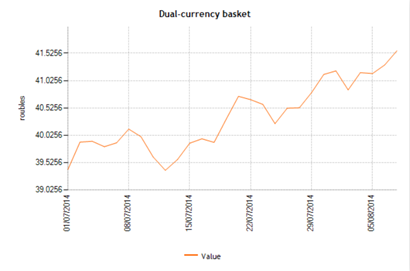
\includegraphics[scale=0.7]{img/dual_currency_busket}
\caption{The values of the dual currency basket calculated by The Central Bank of Russian Federation}
\end{figure}
Source: The Central Bank of Russian Federation. 2016. http://www.cbr.ru/
\end{frame}

\end{document}